\documentclass[a4paper, 12pt]{article}

\usepackage[left=2cm,right=2cm,
top=2cm,bottom=2cm,bindingoffset=0cm]{geometry}

\usepackage[T2A]{fontenc}
\usepackage[utf8]{inputenc}
\usepackage{color}
\usepackage{graphicx}
\usepackage{caption}
\usepackage{listings}
\usepackage{subcaption}
\usepackage{tikz}
\usepackage{float}
\usepackage[english, russian]{babel}
\usepackage{amsmath,amsfonts,amssymb,amsthm,mathtools}
\usepackage{lscape}

\begin{document}
	\begin{center}
		\textbf{\textit{Задание}}
	\end{center}
	
	\begin{enumerate}
		\item Построить функции формы с помощью аппроксимации Лагранжа и Сирендипова семейства для квадратичного четырехугольного элемента 
		\item Вычислить производные от функций форм $\dfrac{\partial N_i}{\partial x}, \dfrac{\partial N_i}{\partial y}$
		\item Вычислить интеграл $ \iint\limits_S \left(\dfrac{\partial N_i}{\partial x}\cdot \dfrac{\partial N_i}{\partial y}\right)\, dS$
	\end{enumerate}
	\begin{figure}[H]
		\centering
		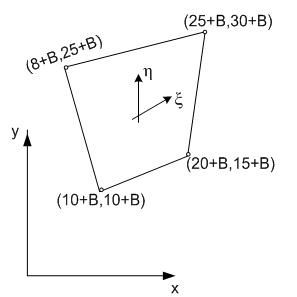
\includegraphics[width=0.3\linewidth]{task.png}
	\end{figure}

	\begin{center}
		\textbf{\textit{Решение}}
		
		\textit{\textbf{В = 15}}
	\end{center}
	\begin{figure}[H]
		\centering
		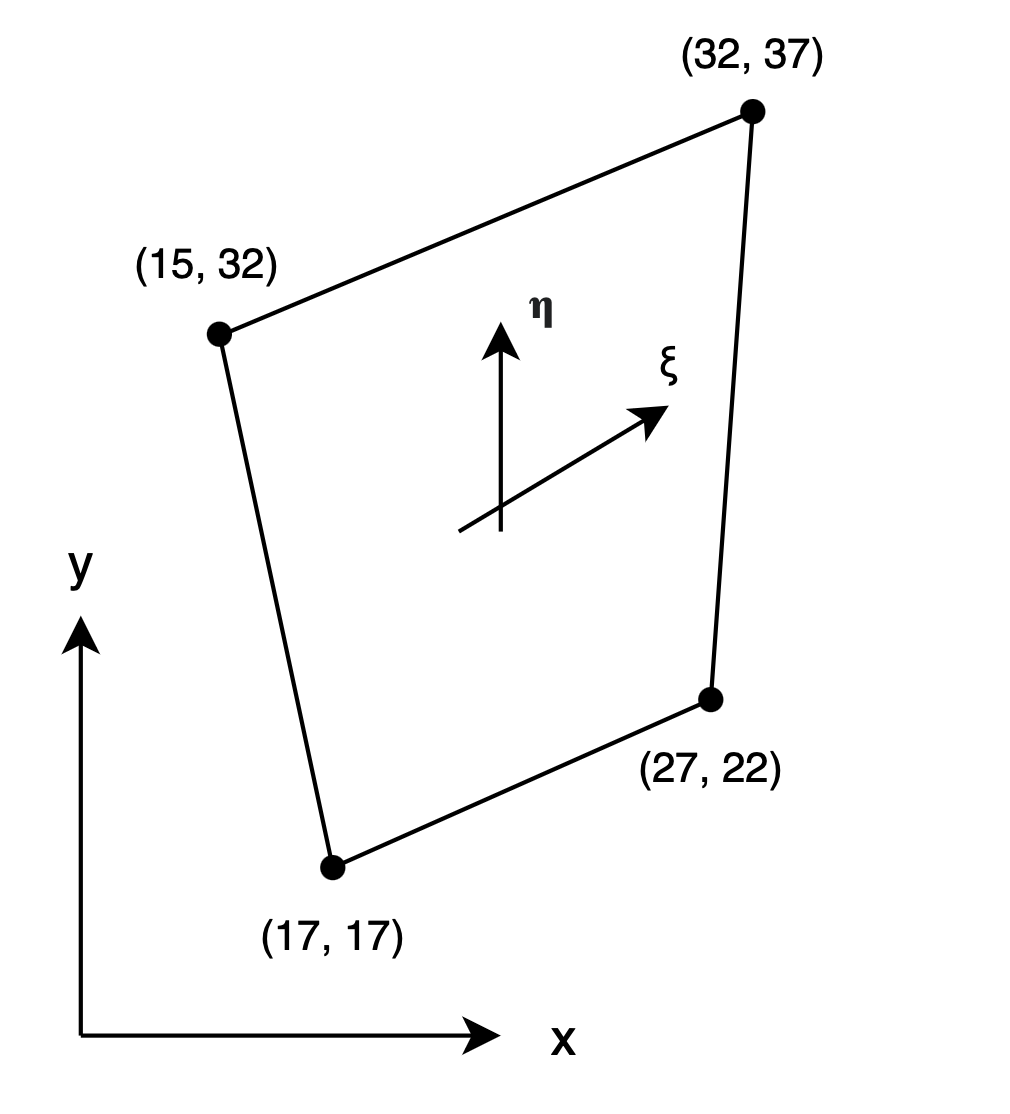
\includegraphics[width=0.3\linewidth]{mytask.png}
	\end{figure}
	
	В естественной системе координат:
	\begin{figure}[H]
		\centering
		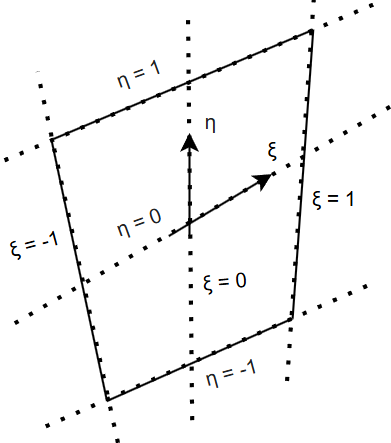
\includegraphics[width=0.3\linewidth]{ncs.png}
	\end{figure}
	
\end{document}